\chapter{Analyse et spécification}
\epigraph{If a student takes the whole series of my folklore courses including the graduate seminars, he or she should learn something about fieldwork, something about bibliography, something about how to carry out library research, and something about how to publish that research.}{Alan Dundes}
\subparagraph{}
Ce chapitre procède à une analyse de l'existant au sein du département commercial-marketing au début de notre stage et y relève des points de critiques auxquels nous proposons une architecture applicative en guise de solution. Ceci après avoir fait un tour d'horizon des recherches scientifiques ayant adressé des problématiques similaires pour inspirer le cadrage fonctionnel et technique de notre projet.
\cleardoublepage

\section{Analyse de l’existant}
\subsection{Description du processus d'analyse du marché}
L’utilisation des données au sein de la direction commerciale est basée sur le partage
d’information concernant les marchés cibles de l’OCP. La répartition des chargés d'études de
marché selon les continents du globe crée un besoin spécifique pour chaque analyste marché.
Pour déterminer les prix de vente ou négocier les prix d’achat des matières premières plusieurs
réunions quotidiennes sont indispensables. Lors de ces réunions des perspectives sur le marché sont partagés entre les analystes OCP à la base de leur revue des données qui leur parviennent par les prestataires d'informations et les solution de Business Intelligence mises en place par nos prédécesseurs(\cite{NACER,CHEMLAL}). L'objectif de notre stage est d'emmener les capacités Business Intelligence du simple reporting à la proposition de mécanismes prévisionnels fluidifiant le processus d'arbitrage quant aux volumes et prix de production. Nous résumons ce processus par la figure \ref{fig:exista} ci-dessous.
			\begin{figure}[H]
					\centering
					\fbox{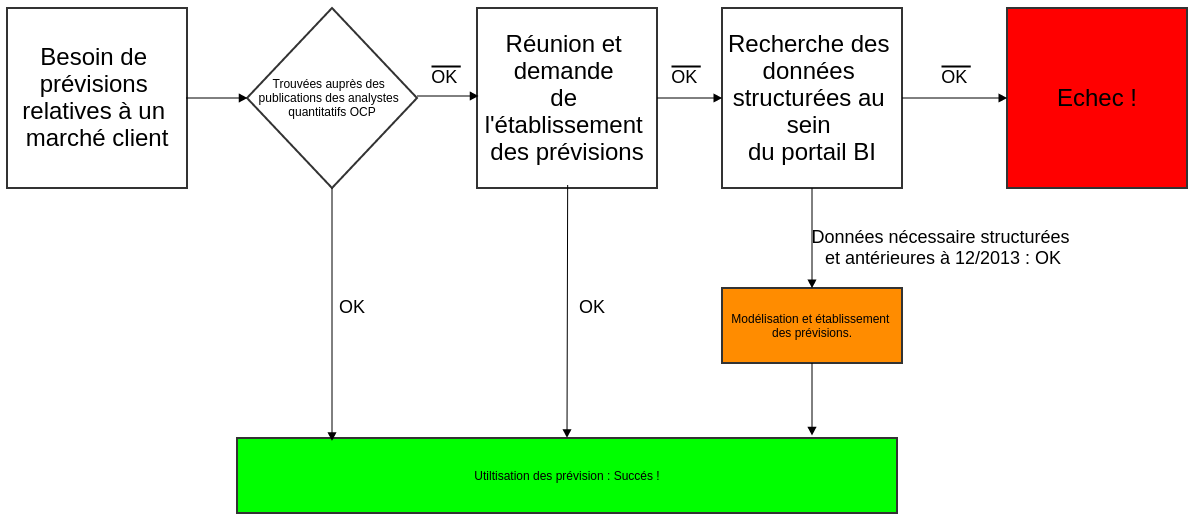
\includegraphics[width=\textwidth]{ch2-images/exist}}
				\caption{Description du processus d'analyse du marché}
				\label{fig:exista}
			\end{figure}
\subsection{Critique de l'existant}
En se basant sur l’utilisation actuelle des fichiers, nous avons constaté que les analystes passent un temps important à structurer les données avant leur utilisation pour émettre des perspectives du marché en cas de non existence de prévision souhaitées.
\par
Après avoir structuré les données, l’analyste les transforme en information en les éditant sous Excel. Cette transformation, des fois manuelle, peut engendrer plusieurs erreurs qui sont liées à la protection de fichiers PDF ou leur mise en page sans compter le temps gaspillé par ces routines non automatisées. Cette tâche est fastidieuse et sera amplement détaillée dans la section \ref{humanpdf}.
\par
Les données ainsi compilées, elle sont utilisées aux fins de modélisation. A la réapparition d'un scénario similaire concernant un client différent, le processus est à nouveau repris avec les mêmes hypothèses.
\par
Au vu de ce processus, nous avons pu identifier plusieurs problèmes parmi lesquels nous citons :
\begin{itemize}
	\item Inexistence d'outils d'aide à la décision intégrant des mécanismes prévisionnels.
	\item Les données rapportés par le système BI en place datte parfois de fin décembre 2013.
	\item Le traitement des données prend un temps important ce qui gêne la compréhension
mutuelle et la collaboration des analystes.
	\item Le niveau d'exploitabilité des données est très bas.
	\item L’absence d’un système d’historisation des données brutes ainsi que les résultats des
analyses.
	\item L’absence de la structuration automatique des données brutes, notamment les .pdf.
	\item Faible fiabilité des données saisies manuellement.
	\item Risque de perte d’information à toute étape du processus.
\end{itemize}
\section{Revue de littérature}
\subsection{Qu'est ce que le Data Mining ?}
La fouille de données, français pour le "Data Mining" est le processus de recherche et de découverte d'auparavant inconnus et potentiellement intéressants modèles dans les grands ensembles de données \cite{def-DM}. L'information 'minée' est typiquement représentée par un modèle de la structure sémantique de l'ensemble de données, où le modèle peut être utilisé sur de nouvelles données à des fins de prédiction ou de classification. Alternativement, des experts humains du métier en question peuvent choisir d'examiner manuellement le modèle, à la recherche d'éléments qui expliqueraient des caractéristiques précédemment mal comprises ou inconnues du domaine d'étude.
\par
Brynjolfsson, Hitt, et Kim\cite{data-driven-des} ont mené des recherches empiriques et ont conclu que la performance des organisations est directement liée à leur capacité à prendre des décisions dirigées par les données. Il est donc important de comprendre les facteurs de succès nécessaires pour adopter des techniques de fouilles de données dans les organisations. En plus des défis techniques, le data mining présente également un ensemble de défis de gestion. Le plus important parmi ceux-ci est la nouvellement acquise capacité de l'organisation à prendre des décisions basées sur les données et donc l'éloigne de la prise de décision basée sur l'intuition. Le leadership, la gestion des talents, de la technologie, la prise de décisions et de la culture de l'entreprise sont des facteurs essentiels pour réussir à tirer parti des grandes données pour la performance organisationnelle\cite{mcafee12}.\paragraph{}
Du côté agricole, Ashlee Vance de rapporte que l'entreprise innovante, \textit{Climate Corp}, qui utilise des données météorologiques localisées pour prédire les rendements des cultures et utilise ces données pour échafauder des primes d'assurance sur les récoltes sur mesure aux agriculteurs individuels. \textit{Climate Corp} enregistre et analyse plus de 60 ans de données météorologiques, comprenant les précipitations, la température et les conditions du sol avec une granularité de 4 kilomètres de rayon afin d'arriver à des prévisions de rendement des cultures\cite{vince12}.\par
\subsection{Les études de prévisions en matière de fertilisants}\label{read1}
L'agriculture est étroitement liée à la sécurité alimentaire des nations, un grand nombre de recherches ont été menées par des organismes gouvernementaux pour assurer un avenir agricole durable et productif. La majorité des prévisions dans les utilisations agricoles utilisent des modélisations économétriques. Cela implique l'utilisation de variables exogènes pour prévoir les rendements des cultures,la consommation des engrais, etc. Nous sommes particulièrement intéressés par les recherches liées à la prévision de la consommation d'engrais puisqu'elles se rapportent à notre problématique.\par
Les premiers travaux connus en matière de prévision de la consommation des engrais ont été réalisés par Vail \cite{Vail27}, puis par
Mehring et Shaw \cite{Mehr44}. Ils ont essayé d'étudier la relation entre la consommation par hectare d'azote et entre la valeur des récoltes, la teneur du sol en azote, et la proportion de trésorerie générée
du bétail. Ils ont tous étudié la relation entre les dépenses en engrais avec
le revenu agricole retardé d'une année. Mehring et Shaw ont conclu que les agriculteurs ont toujours tendance à dépenser une proportion constante de leur revenu sur les engrais. Vail n'a trouvé aucune relation significative entre la consommation d'engrais et les prix des engrais.
Zvi Griliches\cite{Zvi58} a réalisé une autre étude de la consommation d'engrais avec l'objectif d'estimer l'élasticité à court et long terme de la demande. Il a constaté que
les changements technologiques qui ont abouti à de nouvelles technologies de production ont conduit à une réduction du prix réel des engrais, ce qui conduit à l'adoption à grande échelle et une utilisation accrue des engrais.
L'hypothèse de Griliches était qu'une augmentation de l'utilisation d'engrais a été principalement entraînée par une baisse du prix de l'engrais par rapport à d'autres intrants agricoles. Il a modelé la consommation d'engrais dans la saison en cours en fonction du prix de l'engrais et la consommation d'engrais de la saison précédente en utilisant les données 1911-1956.\par
La FAO\footnote{Organisation des nations unies pour l'alimentation et l'agriculture} publie une perspective mondiale sur la demande d'engrais et les tendances des autres produits agricoles telles que les rendements des cultures et la production de céréales. Parthasarathy\cite{PAR94} de la FAO a analysé divers facteurs qui influent sur la consommation d'engrais à long et court terme. En plus de facteurs exogène tels que le pouvoir d'achat des agriculteurs, qui est déterminé par le caractère abordable des engrais, et la trésorerie de liquidités des agriculteurs, la disponibilité de l'engrais influence également la consommation. L'infrastructure et une meilleure gestion de la logistique résultent en une plus grande disponibilité du produit au moment du besoin des agriculteurs, ainsi la demande en assurant est convertie en vente. Selon Parthasarathy, en outre à la terre (superficie plantée et récoltée) et le rendement, d'autres facteurs tels que la quantité et la répartition des précipitations, les modes de culture, et la taille des exploitations influent également sur la consommation d'engrais.\\
Dans un rapport plus récent, la FAO a émis ses prévisions de la consommation d'engrais pour 2015 et 2030 et conclue que les intrants agricoles sont étroitement liés au rendement des cultures, et que la croissance de la production est directement gouvernée par les facteurs macro tels que l'augmentation de la population et le revenu par habitant.
La relation positive entre la consommation d'engrais et la production agricole est bien
établie dans les deux pays en développement et développés. Le scénario de base pour la projection des utilisations d'engrais suppose l'utilisation d'engrais liée à la superficie plantée et le rendement. Le modèle était un modèle de régression logistique, où les transformations logarithmiques des variables indépendantes ont été utilisés comme intrants\cite{FAO2000}.\par
Enfin, alors que les travaux de Griliches \cite{Zvi58} ont porté uniquement sur l'utilisation des engrais, Tenkorang \cite{Tenk06} a tenté de prévoir la demande d'engrais global à long terme, similairement au travail effectué par la
FAO. En plus de la prévision de la consommation d'engrais, que la FAO a achevée, Tenkorang a également tenté d'estimer l'équilibre des éléments nutritifs du sol. Puisque notre projet ne portera pas sur l'estimation des éléments nutritifs du sol, nous nous concentrons sur sa méthode d'estimation des engrais. Il a prévu la demande à travers 182 pays divisés en neuf régions, en utilisant les données de 1962 à 2005. Un intéressant
constat est la relation entre les usages d'engrais dans les années suite à une récolte exceptionnelle.
Les agriculteurs ont tendance à avoir le syndrome de \textit{Good Year/Bad Year} où ils sentent qu'une saison à haut rendement est
généralement suivie par un rendement plus faible. Par conséquent, ils manquent peut-être de motivation à prendre des mesures pour augmenter les consommations de fertilisants suite à une bonne année. En conséquence, Tenkorang a modélisé l'utilisation des engrais dans une région et période de temps données en fonction d'une régression linéaire entre la production de la campagne agricole actuelle, la récolte de l'année précédente, la superficie totale cultivée, et une variable fictive\footnote{\textit{Dummy Variable} pour les anglophones.} pour tenir compte de tout changement structurel des utilisation d'engrais. Cependant, puisque que les terres cultivées et le rendement des cultures sont fondamentalement liés, son
modèle souffre de multi-colinéarité. Ceci a été corrigé en supprimant ces variables indépendantes de l'équation en se basant sur le VIF\footnote{Le Facteur de l'Inflation de la Variance quantifie la gravité de multi-colinéarité dans une régressions par méthodes des moindres carrés. Il fournit un indice qui mesure combien la variance d'un coefficient de régression estimé est augmenté en raison de la colinéarité.}. Le modèle final,ajusté pour multi-colinéarité, a réalisé un $R^2$ élevé\footnote{En statistique, le coefficient de détermination $R^2$ est une mesure de la qualité de la prédiction d'une régression linéaire. Il est défini comme 1 moins le ratio entre l'erreur avec les valeurs prédites et la variance des données}, avec pour la majorité des régions, la terre cultivée comme facteur le plus important.\paragraph{}
Ces études mettent en avant deux concepts importants dans les prévisions agricoles. Tout d'abord, la plupart des modèles de prévisions utilisés sont des modèles causaux qui tentent de relier une variable dépendante telle que la demande d'engrais à un ensemble de variables exogènes. Deuxièmement, ces études nous indiquent quelques uns des facteurs de base ou variables indépendantes que nous devrions prendre en compte dans la construction de notre modèle : Des facteurs agraires, climatiques mais aussi socio-économiques.
\section{Compréhension du problème}
	\subsection{Cadrage fonctionnel du projet}
	À la lumière de notre lecture bibliographique, nous procédons à l'établissement de la liste des divers méthodologies de prévisions en nous intéressant particulièrement aux forces et faiblesses de chacune ainsi qu'aux exigences techniques et informationnelles que celles-ci nécessitent. Nous retiendrons deux approches qui constitueront le cadre fonctionnel de notre projet. Les paragraphes suivants rendent compte de cette évaluation.
	\subsubsection{Les étapes d'une prévision}
	La prévision des engrais peut être divisée en trois étapes complémentaires les unes aux autres, à savoir:\begin{enumerate}
	\item l'évaluation du potentiel,
	\item les prévisions de la demande
	\item les prévisions des ventes
	\end{enumerate}
	Pour le gouvernement les deux premières étapes sont importantes. Pour les organisations de commercialisation, les deuxième et troisième étapes sont pertinentes. Le gouvernement souhaite savoir l'écart entre le potentiel et la demande afin de déterminer ce qu'il doit faire pour transformer une partie du potentiel en demande effective. Une entreprise souhaite savoir ce que la demande effective est et quelle part elle peut être satisfaite par les ventes de l'entreprise.\par
	En ce qui concerne la méthodologie de prévision employée, les méthodes de prévision entrent dans l'une des quatre approches de base:\begin{itemize}
	\item Mesure du potentiel par des méthodes agronomiques ou orientées besoins, 
	\item L'analyse et la projection de séries chronologiques,
	\item Modèles causaux,
	\item Approche qualitative.
	\end{itemize}\par
	De par sa nature, la première approche s’intéresse au long terme et est essentiellement idéaliste. Elle nous dit ce que la demande d'engrais pourrait être et non ce que la demande d'engrais est susceptible d'être.\par
	La seconde approche repose sur des données historiques pour analyser et discerner des schémas de la demande pour prévoir l'avenir, l'hypothèse étant que l'avenir est une continuation du passé. Des données fiables sur plusieurs années sont essentielles pour cette approche.\par
	La troisième approche cherche à établir une relation de cause à effet entre la demande d'engrais et d'autres variables indépendantes dans l'environnement du marché des fertilisants. Comme dans le cas de la méthode des séries chronologiques, les données passées sont importantes pour évaluer l'effet de ces facteurs sur la demande. Les deuxième et troisième méthodes ne peuvent pas être utilisées lorsque l'on veut prévoir l'avenir d'un produit qui n'a pas d'historique ou est dans un stade de développement tel qu'aucun modèle ni tendance sont perceptibles. La consommation d'engrais dans de nombreux pays en développement est dans une telle situation.\par
	La quatrième approche utilise des informations qualitatives, y compris des avis d'experts, pour prévoir la demande. Cette approche peut ou peut ne pas considérer le passé. Les approches qualitatives sont utilisées lorsque les informations sont rares ou ne sont pas fiables, comme dans le stade élémentaire du cycle de vie du produit. Ces conditions étant caractéristiques des marchés des engrais dans les pays en développement, les techniques qualitatives sont très utiles. L'utilisation du jugement humain associé à des systèmes de notation transforment les opinions qualitatives en moyens quantitatifs pour les prévisions.
	\subsubsection{L'extension de la tendance via séries chronologiques pour la prévision}
	Une méthode couramment utilisée pour la prévision est l'analyse des données historiques pour discerner l'évolution de la croissance de la demande et de l'étendre à l'avenir pour prévoir la demande. Si les données de plusieurs années de ventes d'engrais sont disponibles et la tendance est relativement stable, il est possible de lire les données antérieures de la "vitesse" actuelle de la croissance de la demande et la mesure dans laquelle la vitesse augmente ou diminue.\par
	L'extension de tendance est effectuée comme suit:
	\begin{itemize}
	\item Les données chronologiques de la demande d'engrais sont répertoriées.
	\item Ces données sont susceptibles d'avoir quatre composantes majeurs. La première reflète la \textit{tendance} qui se réfère à la variation se produisant constamment sur une longue période. La deuxième composante saisit un mouvement cyclique de la demande dont la plupart des produits, y compris les engrais, sont soumis. Comprendre la variation cyclique est utile pour les prévisions à court et moyen terme. Le troisième élément est la \textit{variation saisonnière} au sein de chaque année. La quatrième composante est la perturbation causée par des \textit{événements erratiques et aléatoires}. Grâce à des méthodes statistiques les données de séries chronologiques sont analysées et décomposées en ces quatre composantes et re-combinés pour fournir la formule de prévision.
	\item L'extension de la tendance est déterminée par un ajustement d'une équation mathématique appropriée qui se rapproche de la tendance historique. Par exemple, la tendance peut être linéaire, à savoir une ligne droite, la pente de degré de la ligne droite indiquant la quantité d'augmentation annuelle de la demande. Les tendances peuvent être quadratique ou exponentielle. Les équations mathématiques décrivent le taux représenté par chacune de ces formes de croissance et nous choisissons l'équation minimisant l'erreur à la tendance historique pour calculer la demande future.
	\end{itemize}
	\subsubsection{Les modèles causaux pour la prévision}
	Le modèle causal est ainsi appelé parce qu'il emploie la relation de cause à effet entre la demande d'engrais et les facteurs qui l'affectent. Le modèle ne représente pas la demande d'engrais au fil du temps ou pour un moment particulier, mais présente la demande par rapport à un ensemble de circonstances. Bien que la méthode d'extension de tendance suppose que le temps reflète tous les facteurs, la méthode causale cherche à établir des relations directes entre la demande d'engrais et les facteurs qui l'influencent. Les facteurs influant sur la demande, comme nous l'avons vu dans la section \ref{read1}, comprennent les prix des cultures, les prix des engrais, la disponibilité du crédit, la superficie irriguée, les précipitations, la superficie cultivée en variétés à haut rendement, le modèle de culture,etc. En analysant les données passées, un ensemble de facteurs essentiels qui ont l'effet le plus profond peuvent être sélectionnés et l'effet des facteurs sélectionnés quantifiés et exprimés sous la forme d'équations mathématiques. Pour projeter la demande pour les années à venir, l'état probable de chaque facteur critique sélectionné à ce point de temps doit d'abord être évalué.
	
	Cette méthode est extrêmement complexe, impliquant des équations mathématiques pour exprimer les relations et les inter-relations entre les variables. En outre, la fiabilité n'est pas garantie car elle dépend des prévisions des valeurs des facteurs critiques choisis. Au mieux, il nous dit ce que la demande est susceptible d'être dans un ensemble donné de circonstances, mais il n'y a aucune certitude que cet ensemble de circonstances prévaudra durant les années sous prévisions.
	
	Une condition sine qua non pour l'utilisation de cette méthode est la disponibilité des données, selon la région et la saison, de divers facteurs critiques en plus des données sur la demande d'engrais pendant plusieurs années. Comme mentionné, une sérieuse limitation de la méthode de causalité est que la prévision, à son tour, dépend des indicateurs qui doivent être eux-mêmes projetés.
	\subsection{Cadrage technique du projet}
	\subsubsection{Architecture globale de notre solution}
			\begin{figure}[H]
					\centering
					\fbox{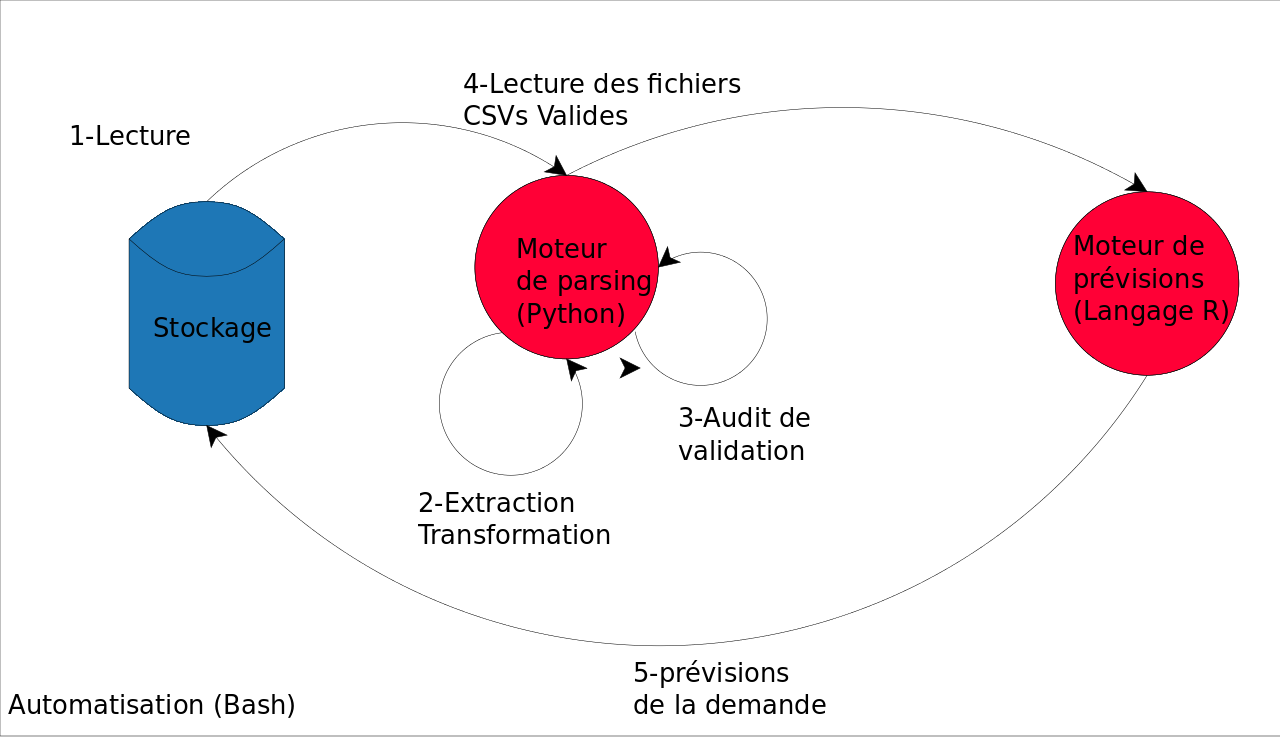
\includegraphics[width=.7\textwidth]{ch2-images/archi}}
					
					\label{fig:archi}
				\caption{Architecture Globale.}
			\end{figure}
	\subsubsection{Outils de réalisation}
		\begin{itemize}
			\item
			\textbf{Le langage de programmation Python : } 
				\begin{itemize}
					\item[$\textasteriskcentered$] Python est un langage de programmation objet, multi-paradigme et multiplate-forme. Il favorise la programmation impérative structurée, fonctionnelle et orientée objet.
					\item[$\textasteriskcentered$] Il est conçu pour optimiser la productivité des programmeurs en offrant des outils de haut niveau et une syntaxe simple à utiliser.
					\item[$\textasteriskcentered$] \textbf{Pourquoi Python dans notre projet ?}
					\begin{itemize}
						\item[\textbf{+}] Calculatrice vectorielle évoluée.
						\item[\textbf{+}] Traitement de fichier texte.
						\item[\textbf{+}] Scripts, ou commandes Unix pour traitements de fichiers par lots.
						\item[\textbf{+}] Langage "Glue" pour enchaîner les traitements par différents programmes.\\\underline{Cas d'utilisation dans notre projet:} Parsing PDF et enregistrement sur fichiers, repris par un code pour structuration des données et traitement.
					\end{itemize}
				\end{itemize}
			\item
			\textbf{Le langage statistique R : } 
				\begin{itemize}
					\item[$\textasteriskcentered$] R est un environnement permettant de faire des analyses statistiques et de produire des graphiques évolués.
					\item[$\textasteriskcentered$] C’est également un langage de programmation complet et mature. Sa licence est open-source, son utilisation est gratuite, même dans le contexte de l’entreprise ou de la formation.
					\item[$\textasteriskcentered$] L’environnement R intègre de nombreuses fonctionnalités pour l'acquisition, le nettoyage et la modélisation de données.
					\item[$\textasteriskcentered$] \textbf{Pourquoi R dans notre projet ?}
					\begin{itemize}
						\item[\textbf{+}] C’est un outil très puissant et très complet, particulièrement bien adapté pour la mise en œuvre informatique de méthodes statistiques. Il est plus difficile d’accès que certains autres logiciels du marché (comme SPSS ou Matlab par exemple), car il n’est pas conçu pour être utilisé à l’aide de «clics» de souris dans des menus. Mais son approche par l'écriture de code informatique pour l'analyse statistique lui confère la flexibilité désiré pour un projet de Data Science.
						\item[\textbf{+}] L’approche est pédagogique puisqu’il faut maîtriser les méthodes statistiques pour parvenir à les mettre en œuvre.
						\item[\textbf{+}] l’outil est très efficace lorsque l’on domine le langage puisque l’on devient alors capable de créer ses propres outils, ce qui permet ainsi d’opérer des analyses très sophistiquées sur les données en retenant tous les avantages de la programmation modulaire dont la ré-utilisabilité et la généricité du code produit.
					\end{itemize}
				\end{itemize}
			\item
			\textbf{Le langage de scripting système BASH : } 
				\begin{itemize}
					\item[$\textasteriskcentered$] Un script BASH est une suite d’instructions, de commandes qui constituent un scénario d'actions. C’est un fichier texte que l’on peut exécuter, c’est à dire, lancer comme une commande.
					\item[$\textasteriskcentered$] \textbf{Pourquoi BASH dans notre projet ?}
					\begin{itemize}
						\item[\textbf{+}] le shell est l'interface de tous les jours en UNIX. Bien connaître son shell permet d'économiser beaucoup d'efforts.
						\item[\textbf{+}] le shell est universel: peu importe le système UNIX, les tâches d'automatisation des appels systèmes privilégient les scripts BASH.
						\item[\textbf{+}] Il est plus aisé de programmer en BASH, par rapport par exemple à C; le Shell n'a pas été conçu pour être minimal ou théoriquement élégant; il a été conçu pour être flexible et pratique. Ainsi, dans bien des cas on va s'en servir pour automatiser les tâches routinières du système.\\
						\underline{Cas d'utilisation dans notre projet:} Automatisation de la création des arborescences de structuration des données à consolider ainsi que les appels systèmes de leur labellisation.
					\end{itemize}
				\end{itemize}
		\end{itemize}
		
		\begin{figure}[H]
			\begin{subfigure}[b]{.3\textwidth}
				\centering
				
\includegraphics[width=\textwidth]{ch2-images/python}
				\caption{Logo Python}
				\label{fig:python}
			\end{subfigure}
			\begin{subfigure}[b]{.3\textwidth}
					\centering
					
\includegraphics[width=.8\textwidth]{ch2-images/R}
					\caption{Logo R}
					\label{fig:R}
			\end{subfigure}
			\begin{subfigure}[b]{.3\textwidth}
					\centering
					
\includegraphics[width=.8\textwidth]{ch2-images/Bash}
					\caption{Logo Bash}
					\label{fig:bash}
			\end{subfigure}
			\caption{Logos des outils utilisés}
		\end{figure}
